\documentclass{standalone}
\usepackage{tikz}
\usetikzlibrary{matrix}

\begin{document}

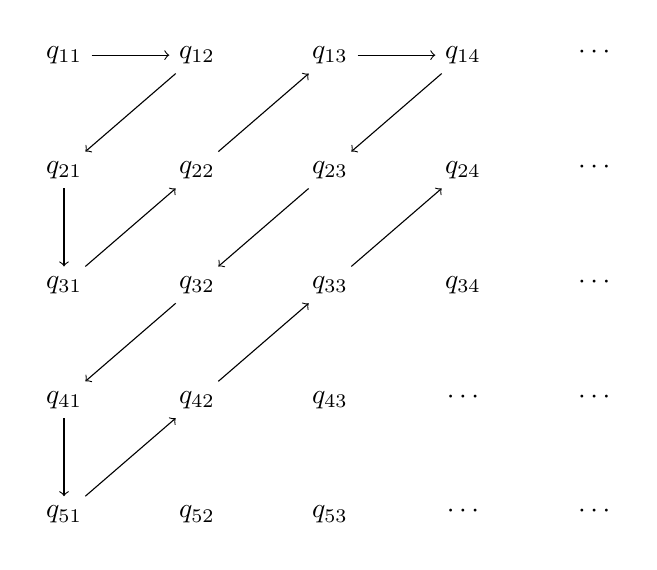
\begin{tikzpicture}
\matrix(m)[matrix of math nodes,column sep=1cm,row sep=1cm]{
    q_{11} & q_{12} & q_{13} & q_{14} & \cdots \\
    q_{21} & q_{22} & q_{23} & q_{24} & \cdots \\
    q_{31} & q_{32} & q_{33} & q_{34} & \cdots \\
    q_{41} & q_{42} & q_{43} & \cdots & \cdots \\
    q_{51} & q_{52} & q_{53} & \cdots & \cdots \\
};

\draw[->]
         (m-1-1)edge(m-1-2)
         (m-1-2)edge(m-2-1)
         (m-2-1)edge(m-3-1)
         (m-3-1)edge(m-2-2)
         (m-2-2)edge(m-1-3)
         (m-1-3)edge(m-1-4)
         (m-1-4)edge(m-2-3)
         (m-2-3)edge(m-3-2)
         (m-3-2)edge(m-4-1)
         (m-4-1)edge(m-5-1)
         (m-5-1)edge(m-4-2)
         (m-4-2)edge(m-3-3)
         (m-3-3)edge(m-2-4);
\end{tikzpicture}\end{document}